\chapter{Introduction}
% awaken the reader’s interest with general information about soccer analysis or sport analysis in general and explain the context
Nowadays sport is more than what it seems to be. Competitive physical activities at the highest level like Soccer, American Football, Tennis or the Olympic Games count to the most-watched television broadcasts. FIFA announced that more than half the world joined an official broadcast of the World Cup 2018 in Russia \cite{worldcup}. Due to the evolving technologies as high resolution cameras and super computers, it's not surprising that an interesting field of computer visualization has evolved from them. 

Tools have been developed for the large number of viewers to bring them closer to the action. Intel True View end-to-end technology solution \cite{intel} makes it possible to render 360-degree replays to give the spectator the feeling of standing on the pitch himself. Other tools like the Vizrt's sports graphics and analysis tools \cite{vizrt} also provides data driven augmented reality but also enables the application for advanced analysis.

\begin{figure}[h]
	\centering
	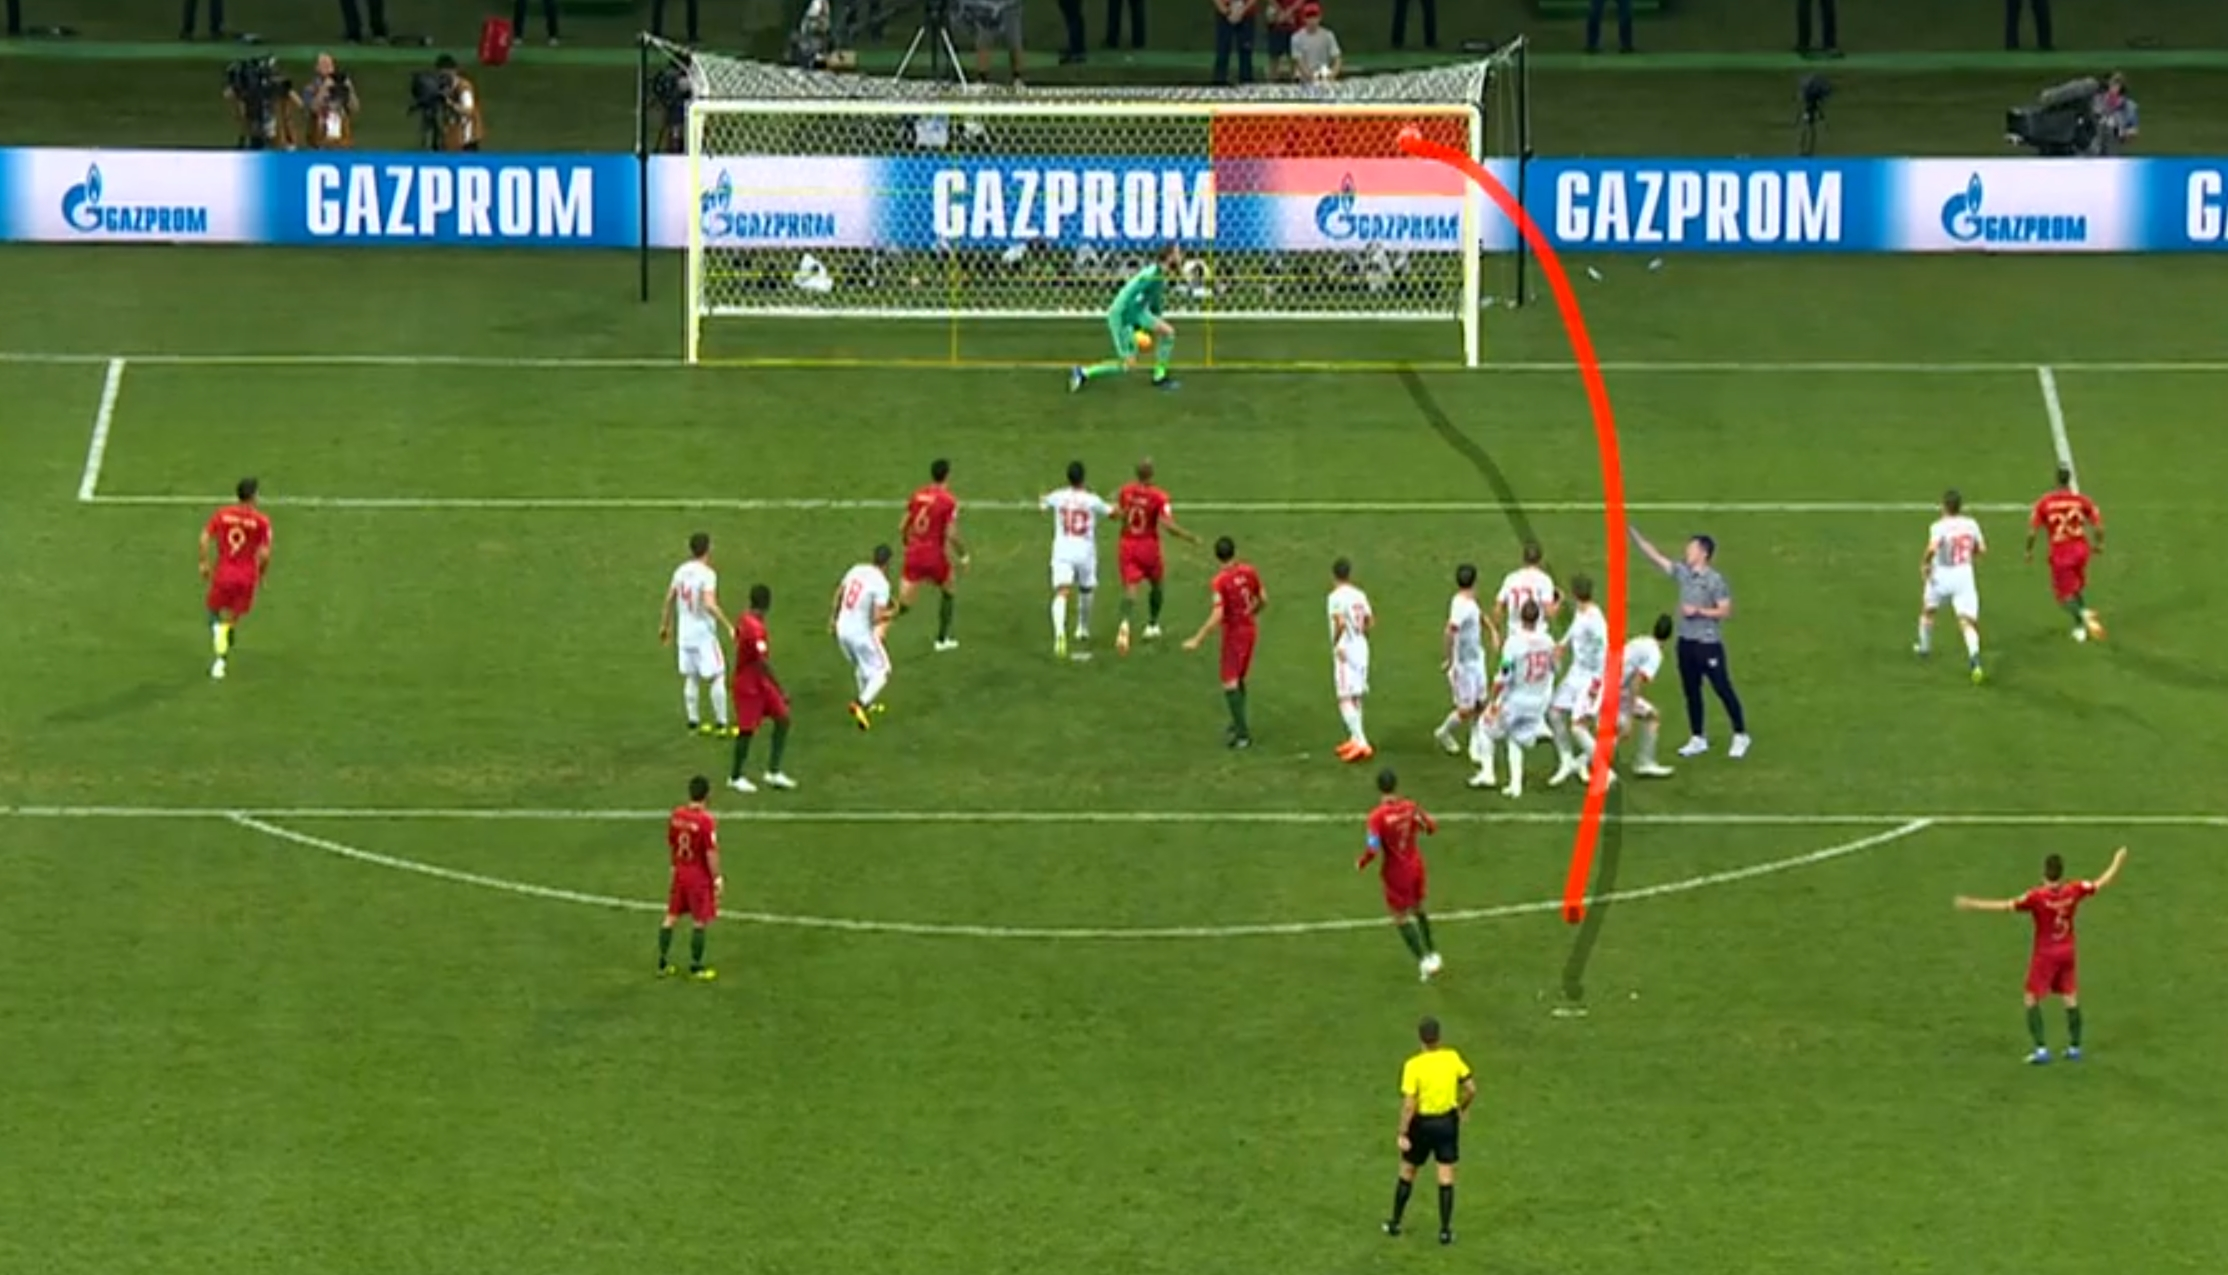
\includegraphics[width=0.8\textwidth]{./images/freekick.jpg}
	\captionsource{Freekick Analysis and Visualization example from Vizrt's sports graphics and analysis tool.\newline}{\cite{vizrt}}
	\label{fig:freekick}
\end{figure}
This leads to the second large field of application of these technologies. Advanced analysis through Visual Computing in sports is important for teams but also for the referee and the audience. The teams try to improve their tactics based on statistics or to learn from past mistakes. Interested spectators are also fascinated by facts from the statistics such as the number of shots at the goal of both teams in soccer. But it also has an impact on the game. The simplest example is the video assistant referee, he draws the referee's attention to a questionable situation and gives him the opportunity to look at the scene again. Obviously this example does not include any Visual Computing theory but is simply a review of the camera recordings.   Another example with computer vision based technology is the Hawk-Eye ball tracking in tennis \cite{hawk}. This allows the trajectory of a ball to be tracked purely from video in order to decide if the ball was in or out. Normally they are so called line umpire which are responsible to call the ball out. By the Hawk-Eye system there was a new opportunity for the players, if they think the ball landed in they can challenge the call of the line umpire. This challenge is then performed using the Hawk-Eye system and the result displayed on the screens in the stadium to be visible to all and to provide clarity. 




\section{Focus of this Work}
% What is the scope of your work? state briefly the focus of the work
% - whats possible with state of the art methods (feasibility study)
The swiss national soccer team approached the computer science department in order to explore state-of-the-art computer vision and visualization technology to analyze soccer games to generate and visualize player statistics and new performance measures of players or teams. The goal of this thesis was to extend the existing two-dimensional tracking system to three dimensions, thus opening up new possibilities. If, for example, not only the position on the pitch is known for each player, but also a three-dimensional skeleton model, this makes it possible to make a statement about the angle of view of the respective player.

\subsection{Thesis Organization}
% helps the reader to pick the interesting points by providing a small text
% explain the related work section and how it's used in the method section
The thesis is structured in the following manner. Chapter \ref{chap:relatedWork} explains other work and discusses the differences to this approach or the similarities that are used in the same fashion in this work. Afterwards the method of this thesis is explained in detail, with a short overview in the next section. The different results are presented and described in chapter \ref{chap:results} and at the end are some conclusions and what could be further improved in the work.

\subsection{Outlook on the Method}
% give an overview of the main points of your thesis what to expect
Available was the video material from multiple TV cameras which pan and zoom during the match and the two-dimensional tracking data. In chapter \ref{chap:method} each step is explained in more detail, but to give you a rough overview:
\begin{itemize}
	\item In order to fit skeleton models to all players in 3D space, stable skeleton joint positions in 2D images had to be estimated with OpenPose. \cite{openpose}. 
	\item The camera calibrations were additionally necessary in order to be able to fuse the 2D positions.
	\item For the multi-view aggregation the extended Kalman Filter was used.
\end{itemize}

